\documentclass[12pt,a4paper]{article}
\usepackage[utf8]{inputenc}
\usepackage{amsmath}
\usepackage{amsfonts}
\usepackage{amssymb}
\usepackage{graphicx}
\usepackage[margin=0.5in]{geometry}

\graphicspath{{./images/}}
\author{Oleg Loshkin}
\title{\textbf{CSC}\\Convertible Scene Creator\\\textbf{Technical Document}}

\begin{document}

\maketitle
\section{Introduction}
	\begin{itemize}
		\item \textbf{Project's Context}
		\\As part of the game programming cursus at SAE Institute Geneva, for the \textbf{technical module GPR5100.2}, students of the second year must \textbf{assist students from the third year in completing their bachelor’s project.}\\\\
		This year, the third year's \textbf{PokFamily team} develops a \textbf{video game for the Switch} and PC using a tailored \textbf{in-house engine}.\\Second year students must \textbf{assist them} by creating various \textbf{tools they will need} in order to create their game.\\\\
		This document describes the functioning of the \textbf{Convertible Scene Creator} tool, \textbf{CSC} for short.
		
		\item \textbf{Project's Goals}
			\begin{itemize}
				\item Create a useful tool that the PokFamily team will use to create their video game.
				
				\item Learn to work in a non-academic environment in a team that depends on the student’s performance.
				
			\end{itemize}
			
		\item \textbf{Specific Problem}
		\\The PokFamily team uses the \textbf{Unity engine as an external editor}. The PokFamily team needs a tool to \textbf{export Unity scenes and prefabs} that may then be used inside the PokEngine.
	\end{itemize}
\newpage

\section{Requirements}
This project’s requirements have two origins:
\begin{itemize}
	\item \textbf{Academic requirements}
		\begin{itemize}
			\item The task given by the team has been understood and done in time.
			
			\item The tool is maintained by the student after the tool's completion.
			
			\item The tool must be user-friendly.
			
			\item The student understands how to manage data.
			
			\item The student understands how a game engine interfaces with a game engine editor.
			
			\item The student has organized himself and his work in a way to facilitate the work of others.
			
			\item The tool’s performance is reasonable.
			
			\item The implementation is appropriately sophisticated.
			
			\item The student understands the implications of non-academic teamwork.
			
		\end{itemize}
	\item \textbf{Pragmatic requirements}
		\begin{itemize}
			\item Convert Unity scene and prefab files to files readable by the PokEngine's parser via UPDC.
			
			\item The user must be able to interact with the tool via Unity.
			
			\item The code must satisfy the quality and style expected by the team. C++ coding style is defined in the Coding Style Document. C\# coding style is defined in UnityWorkOrganization document.
			
			\item The student must communicate with the team appropriately and be dependable.
			
	\end{itemize}
\end{itemize}
%\newpage

\section{Technologies Used}
\begin{itemize}
	\item \textbf{PokEngine}\\
		The \textbf{PokEngine} is the game engine developed by the PokFamily team. The engine is \textbf{written with C++ standard 2014} and \textbf{partly C++ standard 2014} for code running on the Nintendo Switch.\\
The engine has a parser that is capable of reading JSON files. This parser is used to import data exported from Unity with UPDC.

	\item \textbf{Unity 2019.1.10f}\\
		Unity 2019.1.10f is used as an \textbf{external editor}.
	
	\item \textbf{Visual Studio 2017}\\
		Visual Studio 2017 is used for development of the PokEngine.
	
	\item \textbf{Git}\\
		\textbf{github.com} is used for versioning for the \textbf{PokEngine source code}. \textbf{gitlab.com} is used for versioning for the \textbf{Unity prototype source code}. Git bash is used for most interactions with the git framework. Merge conflicts are solved manually via text editor and git bash.		
\end{itemize}

\section{UML Diagram}
\begin{center}
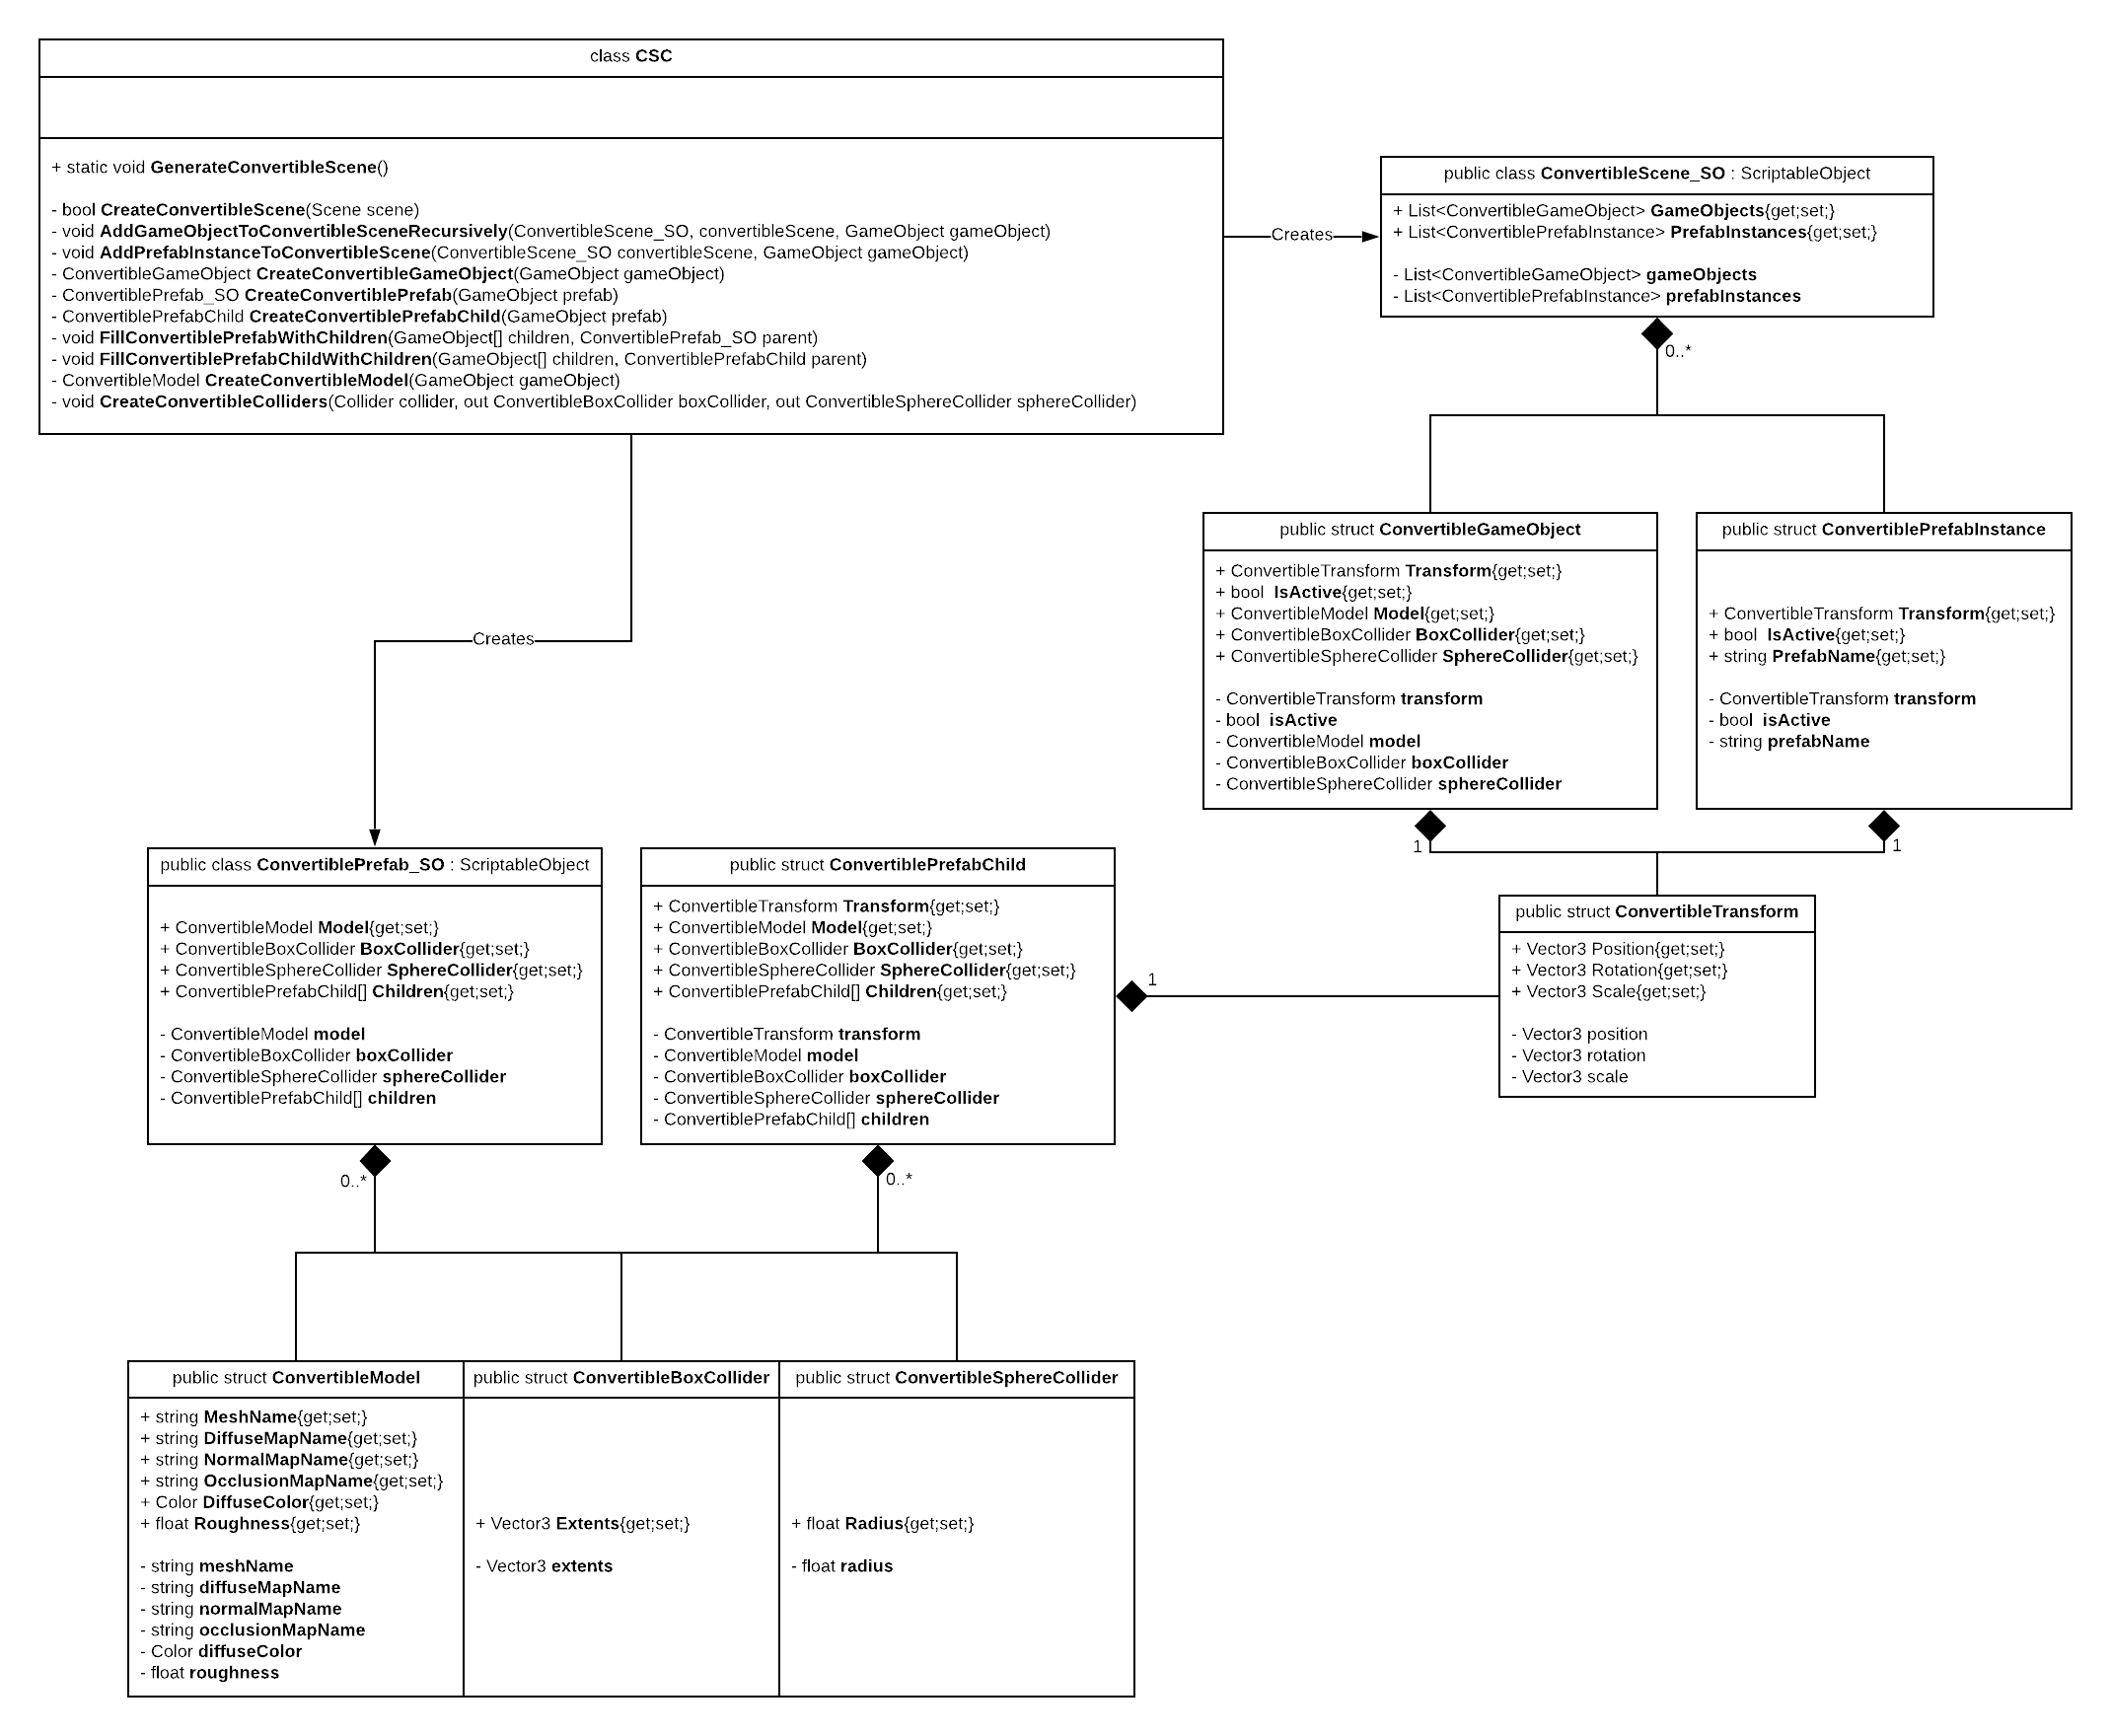
\includegraphics[scale=0.25]{CSCUML}
\end{center}
%\newpage
\textbf{CSC's sole purpose is to create convertible .asset files} by using ScriptableObjects as is described in UPDC's documentation. The \textbf{user's only point of interaction} with the tool is a simple \textbf{drop down menu button} that launches the conversion by taking the currently active scene as input.

\section{Interaction with Overall Project}
\begin{center}
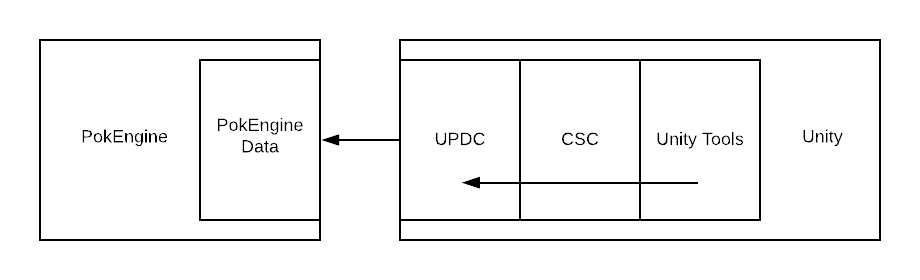
\includegraphics[scale=0.5]{CSCLocation}
\end{center}
\textbf{CSC integrates with UPDC to export scenes and prefabs}. As such, it interacts with Unity's database from which it creates .asset files for UPDC to export.

\section{Exporting Prefabs}
Upon the game designer's request, \textbf{this tool needed to be able to export Unity's prefabs}. This has surprisingly proven to be a challenge.\\\\
Storing whole prefabs in the \texttt{ConvertibleScene\_SO} file would not have made sense since the whole point of a prefab is to define it once, and reference it later wherever it showed up.\\ From this came \textbf{the separation between the \texttt{ConvertiblePrefab\_SO} class}, a ScriptableObject inheriting class \textbf{compatible with UPDC}, and \textbf{the struct \texttt{ConvertiblePrefabInstance}} which is \textbf{a serializable data structure} that is stored in a \texttt{ConvertibleScene\_SO} and that \textbf{references an existing \texttt{ConvertiblePrefab\_SO}.}\\\\
\textbf{More distinctions} were needed to be made \textbf{between GameObjects composing a prefab} however. \textbf{A \texttt{ConvertiblePrefabInstance} has a transform field whereas a \texttt{ConvertiblePrefab\_SO} does not.} This makes sense since an instance of a prefab will have a defined position, rotation and scale relative to a scene, but will not have those by itself.\\
This implies however that \textbf{a \texttt{ConvertiblePrefab\_SO} cannot have other \texttt{ConvertiblePrefab\_SO}'s as children}: these do need to have a transform to define their positions, rotations and scales relative to their parent. From this need, was created \textbf{the \texttt{ConvertiblePrefabChild} struct}.

\section{(Not) Tackling Polymorphism}
In the final JSON files generated by UPDC of \texttt{ConvertiblePrefab\_SO}'s, you will notice the presence of \textbf{two fields for colliders: one for a boxCollider and another for a sphereCollider}. This is due to the fact that C\# does not support polymorphism of struct data types.\\\\
This combined with the fact that Unity's JSONUtility is used by UPDC to generate JSON files rather than a custom build parser results in the inability to represent polymorphism in the JSON files, hence the presence of both types of colliders simultaneously rather than only one collider of particular type or less.

\section{Exporting Models}
\textbf{Unity uses} a combination of \textbf{Meshes and Materials to represent 3D objects}. \textbf{PokEngine uses Models} instead, which combine the functionalities of both. CSC therefore does the work of reading the relevant data from these both data structures to create a serializable struct that corresponds to the format expected by the PokEngine.

\section{Integrating with ProBuilder}
\textbf{ProBuilder was used in the designing of the prototype of the game on Unity}. It is a very powerful tool for prototyping, however it does not easily expose the meshes it generates.\\\\
While it is possible to retrieve them and save them to a specific location in the Unity's project from where they can be accessible by other tools, doing so links the ProBuilder scripts located in a particular scene to those specific meshes. This could lead to version control conflicts.\\
As a workaround, \textbf{CSC} instead \textbf{generates copies of the meshes used by ProBuilder} for it's own use, leaving ProBuilder scripts intact.\\
\textbf{This does come at the cost of extra space being used on disk.}

\section{Potential Improvements}
\begin{itemize}
\item The prefab exportation had been done in a rush, the current implementation has a lot of room for improvement:
\begin{itemize}
\item There are way too many data structures defined to separate between different types of prefab objects, there must be a more elegant way to represent them.
\item For each instance of a given prefab in a Unity scene, a new \texttt{ConvertiblePrefab\_SO} .asset is generated. This defeats the whole purpose or having prefabs in the first place. A system would need to be implemented to prevent the generation of identical convertible prefabs.
\end{itemize}
\item While exportation of ProBuilder meshes is functional, it is implemented in a way as to duplicate already existing meshes. This is a behaviour that could be improved.
\item As a consequence of UPDC's implementation, polymorphism is not handled. A redesign of UPDC might make the implementation of collider exportation more elegant.
\end{itemize}

\section{Summary}
\textbf{The CSC tool provides the user with an easy way to convert a Unity scene and prefabs located inside into formats readable by PokEngine's parser via the use of UPDC.}\\\\
While implementation transparency of the C\# language and Unity's own systems may be beneficial when it comes to superficial tasks, in this case, it has proven to be a hurdle instead.\\
\textbf{Polymorphism, data structures abstractions and data serialization is a problematic mix} I have been confronted with for the first time during this project and the creation of this tool has shown me \textbf{key areas of knowledge that I need to be more mindful of}.

\end{document}
